\chapter{In-memory Inverted Index}
\lhead{Chapter 5. \emph{In-memory Inverted Index}} % this is for the header on each page - perhaps a shortened title
For text retrieval systems, the assumption that all data structures reside in main memory is increasingly common. To achieve optimal performance, we adopted a state-of-art in-memory inverted index --- Zambezi~\cite{Asadi_Lin_IRJ2012,Asadi_Lin_TOIS2013,Asadi_etal_TKDE2013,Asadi_Lin_SIGIR2013}. Zambezi was originally designed for twitter's real-time search. It supports incremental index and several retrieval algorithms. In addition, we applied some enhancements to make it more versatile.

\section{Zambezi}

\subsection{Basic Incremental Indexing Algorithm}
\label{section:algo:basic}

\begin{figure*}[t]
  \begin{center}
    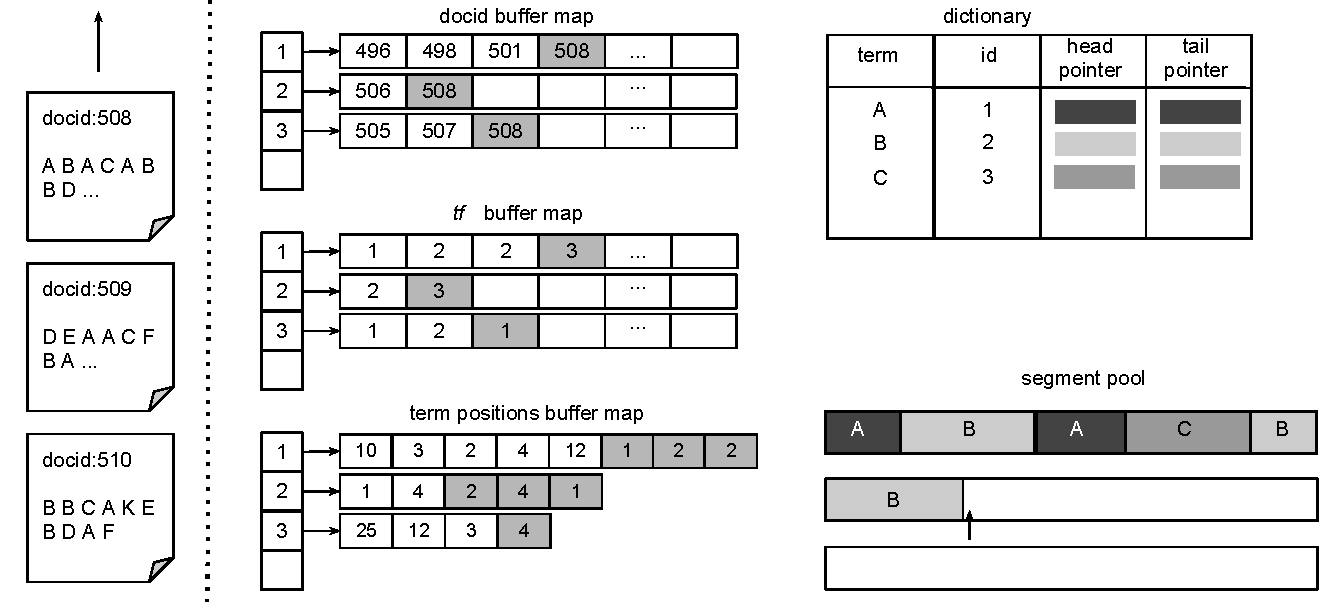
\includegraphics[width=0.8\textwidth]{Figures/IndexStructure.pdf}
  \end{center}
  \caption{A snapshot of our indexing algorithm. In the middle we have buffer maps for storing docids, \textit{tf}s, and term positions: the gray areas show elements inserted for document 508, the current one to be indexed. Once the buffer for a term fills up, an inverted list segmented is assembled and added to the end of the segment pool and linked to the previous segment via addressing pointers. The dictionary maps from terms to term ids and holds pointers to the head and tail of the inverted list segments in the segment pool.
  \label{figure:indexStructure}}
\end{figure*}

Our indexer consists of three main components, depicted in Figure~\ref{figure:indexStructure}: the dictionary, buffer maps, and the segment pool. The basic indexing approach is to accumulate postings in the buffer maps in an uncompressed form until the buffer fills up, and then to ``flush'' the contents to the segment pool, where the final compressed postings lists reside. Note that in this approach the inverted lists are discontiguous; we return to address this issue in Section~\ref{section:algo:contiguity}.

The dictionary is implemented as a hash table with a bit-wise hash function~\cite{RamakrishnaDASFAA1997} and the move-to-front technique~\cite{WilliamsSPE2001}, mapping terms (strings) to integers term ids (see~\cite{ZobelIPL2001} for a study that compares this to other approaches). There is nothing noteworthy about our dictionary implementation, and we claim no novelty in this design. The dictionary additionally holds the document frequency (\textit{df}) for each term, as well as a head and tail pointer into the segment pool (more details below). In our implementation, term ids are assigned sequentially as we encounter new terms.

A \textit{buffer map} is a one-to-one mapping from term ids to arrays of integers (the buffers). Since term ids increase monotonically, a buffer map can be implemented as an array of pointers, where each index position corresponds to a term id, and the pointer points to the associated buffer. The array of pointers is dynamically expanded to accommodate more terms as needed. To construct a positional index, we build three buffer maps: the document id (docid) map, the term frequency (\textit{tf}) map, and the term positions map. As the names suggest, the docid map accumulates the document ids of arriving documents, the \textit{tf} map holds term frequencies, and the term positions map holds term positions. There is a one-to-one correspondence between entries in the docid map and entries in the \textit{tf} map (for each term that occurs in a document, there is exactly one term frequency), but a one-to-many correspondence between entries in the docid map and entries in the term positions map (there are as many 
term positions in each document as the term frequency).

In the indexing loop, the algorithm receives an input document, parses it to gather all term frequencies and term positions (relative to the current document, starting from one) for all unique terms, and then iterates over these unique terms, inserting the relevant information into each buffer map. Whenever we encounter a new term, the algorithm initializes an empty buffer in each buffer map for the corresponding term id. Initially, the buffer size is set to the block size $b$ that will eventually be used to compressed the data (leaving aside an optimization we introduce below to control the vocabulary size). Following best practice today, we use PForDelta~\cite{ZukowskiICDE2006,Yan_etal_WWW2009}, with the recommended block size of $b=128$. The term positions map expands one block at a time when it fills up to accommodate more positions. When the docid buffer for a term fills up, we ``flush'' all buffers associated with the term, compressing the docids, term frequencies, and term positions into what we call 
an inverted list segment, described below:

Each inverted list segment begins with a run of docids, gap-compressed using PForDelta; call this $D$. By design, the docids occupy exactly one PForDelta block. Next, we compress the term frequencies using PFor; call this $F$. Note that term frequencies cannot be gap-compressed, so they are left unmodified. Finally, we process the term positions, which are also gap-encoded, relative to the first term position in each document. For example, if in $d_1$ the term was found at positions $[1, 5, 9]$ and in $d_2$ the term was found at positions $[3, 16]$, we would code $[1, 4, 4, 3, 13]$. The term positions can be unambiguously reconstructed from the term frequencies, which provide offsets into the array of term positions. Since the term positions array is likely longer than $b$, the compression block size, the term positions occupy multiple blocks. Call the blocks of term positions $P_1 \ldots P_m$.

Finally, all the data are packed together in a contiguous block of memory as follows:

\begin{displaymath}
  \begin{array}{l}
    \left[\; |D|,\; D,\; |F|,\; F,\; \{ |P_i|,\; P_i \}_{0 \leq i < m} \right] \\
  \end{array}
\end{displaymath}

\noindent where the $|\cdot|$ operator returns the length of its argument. Since all the data are tightly packed in an otherwise undelimited array, we need to explicitly store the lengths of each block to properly decode the data during retrieval.

Each inverted list segment is written at the end of the segment pool, which is where the compressed inverted index ultimately resides. Conceptually, the segment pool is an bounded array with a pointer that keeps track of the current ``end'', but in practice the pool is allocated in large blocks and dynamically expanded as necessary. In order to traverse a term's postings during query evaluation, we need to ``link'' together the discontiguous segments. The first time we write a segment for a term id, we add its address (byte offset in the segment pool) to the dictionary, which serves as the ``head'' pointer (the entry point to postings traversal). In addition, we prepend to each segment the address (byte offset position in the segment pool) of the next segment in the chain. This means that every time we insert a new segment for a term, we have to go back and correct the ``next pointer'' for the last segment. We leave the next pointer blank for a newly-inserted segment to mark the end of the postings list for 
a term; this location is stored in the ``tail pointer'' in the dictionary. Once the indexer has processed all documents, the remaining contents of the buffer maps are flushed to the segment pool in the same manner. By default, we build full positional indexes, but our implementation has an option to disable the term position buffers if desired. In this case, the inverted list segments will be smaller, but other aspects of the algorithm remain exactly the same.

Conceptually speaking, the postings list for each term is a linked list of inverted list segments, where each of the segments is laid out in discontiguous monotonically-increasing byte offset positions in the segment pool and linked together with addressing pointers. Segments corresponding to different terms are arbitrarily interleaved in the segment pool. What are the implications of this design? On the positive side, all data in the segment pool are ``tightly packed'' for maximum efficiency in memory utilization: there are no empty regions and there is no need for special delimiters. During indexing we guarantee that there is no heap fragmentation, which may be a possibility if we simply used \texttt{malloc} to allocate space for each inverted list segment. On the negative side, postings traversal becomes an exercise in pointer chasing across the heap, without any predictable access patterns that will aid in processor pre-fetching across segment boundaries. Thus, as a query evaluation algorithm consumes 
postings, it is likely to encounter a cache miss whenever it reaches the end of a segment, since it has to follow a pointer. On the other hand, it is not entirely clear if this cache miss is a major concern: since PForDelta is block-based, postings are decompressed in blocks even if the inverted lists are contiguously stored in memory.

In addition to ``flushing to memory'' (i.e., the segment pool) as opposed to flushing to disk, the operation of our indexer is fundamentally different from previous designs. In previous approaches, the in-memory buffer is completely flushed when the capacity limit is reached, which means that inverted lists associated with \textit{all} terms are written to disk. In contrast, we only flush data associated with the term id whose buffer has reach capacity.

One final optimization detail: we control the size of the term space by discarding terms that occur fewer than ten times (an adjustable document frequency threshold). This is accomplished as follows: instead of creating a buffer of length $b$ when we first encounter a new term, we first allocate a small buffer equal to the \textit{df} threshold. We buffer postings for new terms until the threshold is reached, after which we know that the term will make it into the final dictionary, and so we reallocate a buffer of length $b$. This two-step process reduces memory usage substantially since there are many rare terms in web collections.

\subsection{Segment Contiguity}
\label{section:algo:contiguity}

It is clear that our baseline indexing algorithm generates discontiguous inverted list segments. In order to create contiguous inverted lists, we would need an algorithm to rearrange the segments once they are written to the segment pool. Following the ``remerging'' idea in disk-based incremental indexing, we might merge multiple discontiguous segments belonging to the same term id and transfer them to another region in memory, repeating if necessary. Alternatively, when writing an inverted segment to the segment pool, we might leave some empty space---but since no pre-allocation policy can be prescient, we will either leave too much empty space (wasting memory) or not leave enough (necessitating further copying). These basic designs have been explored in the context of on-disk incremental indexing, but we argue that the issues become more complex in memory because we do not have an intermediate abstraction of the file---the indexing algorithm must explicitly manage memory addresses. This amounts to 
implementing \texttt{malloc} and \texttt{free} for inverted list segments, which is a non-trivial task.

Before going down this path, however, we first examined the extent to which contiguous segments would improve retrieval efficiency, from better reference locality, pre-fetch cues provided to the processor, etc. Let us assume we have an oracle that tells us exactly how long each inverted list is going to be, so that we can lay out the segments end-to-end, without any wasted memory. We simulate this oracle condition by building the inverted index as normal, and then performing in-memory post-processing to lay out all the inverted list contiguously. Obviously, in a real incremental indexing scenario, this is not a workable option, but this simple experiment allows us to measure the ideal performance from the perspective of query evaluation. Thus, we can establish two retrieval efficiency bounds---the query evaluation time on arbitrarily discontiguous inverted lists (the baseline algorithm) and on contiguous inverted lists (the upper bound on query evaluation speed).

Using these two efficiency bounds as guides, we developed a simple yet effective approach to achieving increasingly better approximations of contiguous postings lists. Instead of moving compressed segments around after they have been added to the segment pool, we change the memory allocation policy for the buffer maps. In the limit, if we increased buffer map sizes so that they are large enough to hold the entire document collection in uncompressed form, it is easy to see how we could build contiguous inverted list segments. As it turns out, we do not need to go to such extremes.

In our strategy, whenever the docid buffer for a term becomes full (and thus compressed and flushed to the segment pool), we expand that term's docid and \textit{tf} buffers by a factor of two (still allowing the term positions buffer to grow as long as necessary). This means that after the first segment of a term is flushed, new docid and \textit{tf} buffers of length $2b$ replace the old ones; after the second flush, the buffer size increases to $4b$, and then $8b$, and so on. When a buffer of size $2^m b$ becomes full, the buffer is broken down to $2^m$ segments, each segment is compressed as described earlier, and all $2^m$ segments are written at the end of the segment pool contiguously. This strategy allows long postings to become increasingly contiguous, without wasting space to pre-allocate large buffers to hold terms that turn out to be rare.

To prevent buffers from growing indefinitely and to control the memory pressure, we set a cap on the length of docid and \textit{tf} buffers. That is, if the cap is set to $2^m b$, then when the buffer size for a term reaches that limit, it is no longer expanded. This means that the maximum number of contiguous segments allowed in the segment pool is $2^m$. We experimentally show that for relatively small values of $m$, around 6 or 7, we achieve query evaluation speeds that are statistically indistinguishable from having an index with fully-contiguous inverted lists (i.e., the oracle condition). The tradeoff of this approach is that we require more transient working memory during the indexing process, and that impacts the size of the collection that we can index. However, we experimentally show that the additional memory requirements for implementing this approach are reasonable. Note that for on-disk incremental indexing algorithms, the strategy of increasing the in-memory buffer size is generally not 
considered since those algorithms operate under an assumption of limited memory. In our case, we are simply changing the allocation between transient working memory for performing document inversion and the final index structures.

\begin{table*}[t]
  \setlength{\tabcolsep}{1.5pt}
  \renewcommand{\arraystretch}{1.5}
  \centering
  \scriptsize
  \begin{tabular}{|c|l||c|c|c|c|c|c|c|c||c|}
    \hline
    & Query & $1b$ & $2b$ & $4b$ & $8b$ & $16b$ & $32b$ & $64b$ & $128b$ & Contiguous\\
    \hline
    \hline
    \multirow{2}{0.15cm}{\rotatebox{90}{\tiny Gov2}}
    & Terabyte & 14.4 ($\pm$0.2) & 14.2 ($\pm$0.1) & 13.9 ($\pm$0.1) & 13.6 ($\pm$0.1)
    & 13.3 ($\pm$0.1) & 13.2 ($\pm$0.1) & 13.1 ($\pm$0.1) & 13.1 ($\pm$0.1) & 13.1 ($\pm$0.1) \\
    & AOL & 20.2 ($\pm$0.4) & 19.7 ($\pm$0.1) & 19.3 ($\pm$0.2) & 19.0 ($\pm$0.3) & 18.8 ($\pm$0.3)
    & 18.7 ($\pm$0.5) & 18.4 ($\pm$0.2) & 18.3 ($\pm$0.1) & 18.2 ($\pm$0.2) \\
    \hline
    \hline
    \multirow{2}{0.15cm}{\rotatebox{90}{\tiny Clue}}
    & Terabyte & 49.7 ($\pm$0.2) & 47.1 ($\pm$0.1) & 45.9 ($\pm$0.4) & 44.4 ($\pm$0.5) &
    42.9 ($\pm$0.4) & 42.0 ($\pm$0.3) & 41.6 ($\pm$0.1) & 41.6 ($\pm$0.4) & 41.3 ($\pm$0.1) \\
                    & AOL & 87.5 ($\pm$1.6) & 83.2 ($\pm$0.5) & 80.7 ($\pm$0.3) & 75.5 ($\pm$0.5)
    & 75.7 ($\pm$0.8) & 75.8 ($\pm$0.3) & 75.2 ($\pm$0.2) & 75.0 ($\pm$0.6) & 75.3 ($\pm$1.2) \\
    \hline
  \end{tabular}
  \caption{Average query latency (in milliseconds) for postings intersection using SvS with different buffer length settings. Results are averaged across 5 trials, reported with 95\% confidence intervals.
  \label{table:queryLatency}}
\end{table*}

\subsection{Query Latency}

Table~\ref{table:queryLatency} summarizes query latency for conjunctive query processing (postings intersection with SvS). The average latency per query is reported in milliseconds across five trials along with 95\% confidence intervals. Each column shows different indexing conditions: $1b$ is the baseline algorithm presented in Section~\ref{section:algo:basic} (linked list of inverted list segments). Each of $\{2, 4, 8 \ldots 128\}b$ represents a different upper bound in the buffer map growing strategy described in Section~\ref{section:algo:contiguity}. The final column marked ``contiguous'' denotes the oracle condition in which all postings are contiguous; this represents the ideal performance.

From these results, we see that, as expected, discontiguous postings lists ($1b$) yield slower query evaluation: on Gov2, queries are approximately 10\% slower, while for ClueWeb09, the performance dropoff ranges from 16\% to 20\%.  For higher values of $b$, we allow the buffer maps to increase in length: at $32b$, query evaluation performance is statistically indistinguishable from the performance upper bound (i.e., confidence intervals overlap). That is, we only need to arrange inverted list segments in relatively small groups of 32 to achieve ideal performance. Later, we quantify the memory requirements of allocating larger buffer maps.

\begin{figure*}[t]
  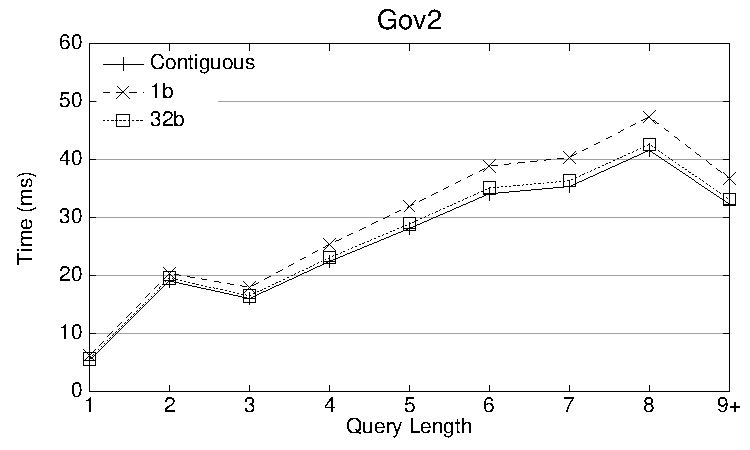
\includegraphics[width=0.49\linewidth]{Figures/latency_gov2_aol.pdf}
  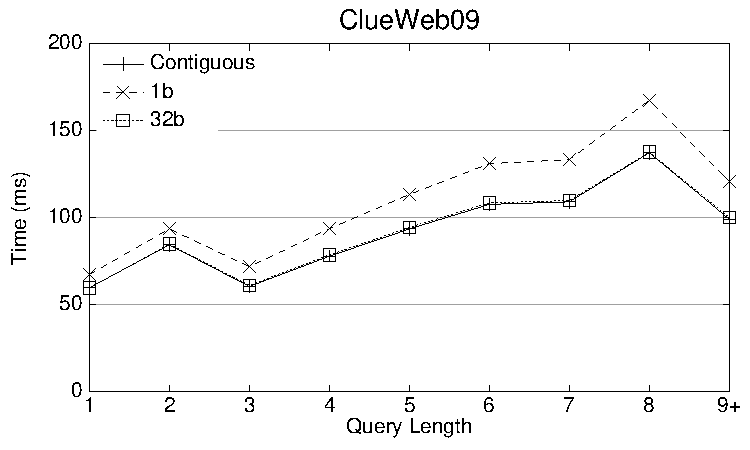
\includegraphics[width=0.49\linewidth]{Figures/latency_clue_aol.pdf}
  \caption{Query latency using SvS for the AOL query set, by query length for different buffer length settings.
  \label{figure:queryLatency}}
\end{figure*}

Figure~\ref{figure:queryLatency} illustrates query latency by query length, for the AOL query set on Gov2 and ClueWeb09, using different conditions. Not surprisingly, the latency gap between contiguous and the $1b$ condition widens for longer queries. On the other hand, the difference between a contiguous index and the $32b$ condition is indistinguishable across all query lengths---the lines practically overlap in the figures.

\begin{table}[t]
  \setlength{\tabcolsep}{3.5pt}
  \centering
  \small
  \begin{tabular}{|c|l||c|c|c|}
    \hline
    & Query & $1b$ & $32b$ & Contiguous\\
    \hline
    \hline
    \multirow{2}{0.1cm}{\rotatebox{90}{\tiny Gov2}}
    & Terabyte & 65.0 ($\pm$0.4) & 62.5 ($\pm$0.8) & 62.0 ($\pm$0.4) \\
    & AOL & 103.5 ($\pm$0.5) & 100.3 ($\pm$0.1) & 100.2 ($\pm$0.4) \\
    \hline
    \hline
    \multirow{2}{0.1cm}{\rotatebox{90}{\tiny Clue}}
    & Terabyte & 150.0 ($\pm$0.5) & 141.1 ($\pm$0.6) & 141.1 ($\pm$0.2) \\
    & AOL & 455.7 ($\pm$5.1) & 434.3 ($\pm$5.8) & 432.6 ($\pm$4.9) \\
    \hline
  \end{tabular}
  \caption{Average query latency (in milliseconds) to retrieve the top 1000 hits in terms of BM25 using WAND (5 trials, with 95\% confidence intervals).
  \label{table:queryLatency:wand}}
\end{table}

For disjunctive query processing, we used the \textsc{Wand} algorithm to retrieve the top 1000 documents using BM25. Table~\ref{table:queryLatency:wand} summarizes these experiments on different collections and queries. For space considerations, we only report results for select buffer length configurations. These results are consistent with the conjunctive processing case. A maximum buffer size of $32b$ yields query latencies that are statistically indistinguishable from a contiguous index. Note that the performance difference between fully-contiguous postings lists and $1b$ discontiguous postings lists is less than 7\%. In other words, there is much less performance degradation than in the SvS case.

As with the conjunctive query processing case, we analyzed query latency by length. The results, however, were not particularly insightful: as expected, query latency increases with length, and the performance differences between the three conditions were so small that the plots essentially overlapped. For this reason, we did not include the corresponding figures here.

\subsection{Memory Usage}

All inverted indexing algorithms require transient working memory to hold intermediate data structures. For on-disk incremental indexing algorithms, previous work has assumed that this working memory is relatively small. In our case, there is no hard limit on the amount of space we can devote to working memory, but space allocated for holding intermediate data takes away from space that can be used to store the final compressed postings lists, which limits the size of the collection that we can index for a fixed server configuration.

At minimum, our buffer maps must hold the most recent $b$ docids, term frequencies, and associated term positions (leaving aside the rare terms optimization in Section~\ref{section:algo:basic}). In our case, we set $b=128$ to match best practices PForDelta block size; any smaller value would compromise decompression performance. In order to increase the contiguity of the inverted list segments, we increase the length of the buffers, as described in Section~\ref{section:algo:contiguity}. This of course increases the space requirements of the buffer maps.

\begin{figure}[t]
  \centering
  \begin{subfigure}[b]{0.45\textwidth}
    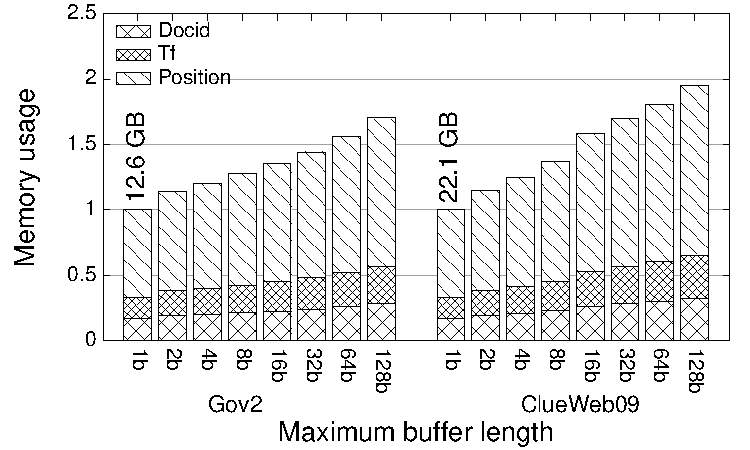
\includegraphics[width=\textwidth]{Figures/memory_usage.pdf}
    \caption{Memory required to hold all buffer maps for different buffer length settings, normalized to the $1b$ setting, on Gov2 and ClueWeb09.
    \label{figure:memoryUsage}}
  \end{subfigure}
  \begin{subfigure}[b]{0.45\textwidth}
    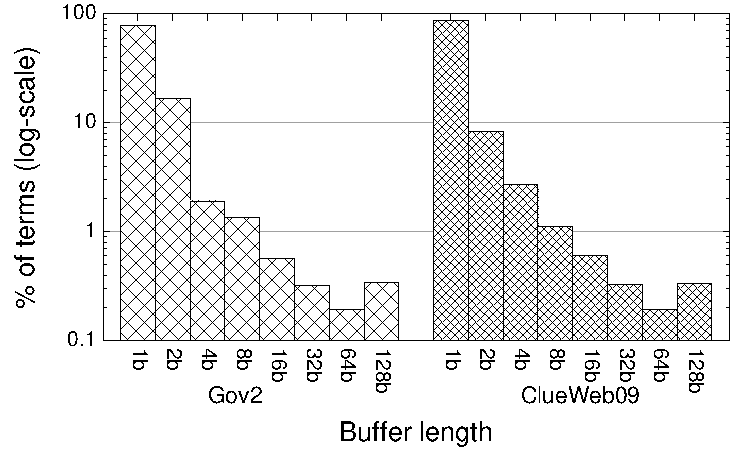
\includegraphics[width=\textwidth]{Figures/buffer_length_32b.pdf}
    \caption{Percentage of terms for which a buffer of length $m \times b$ is required, for different values of $m$, and block size $b=128$.
    \label{figure:bufferLengthDist}}
  \end{subfigure}
  \caption{Memory behavior of buffer maps.}
\end{figure}

Figure~\ref{figure:memoryUsage} shows the maximum size of the buffer maps for different contiguity configurations, broken down by space devoted to docids, term frequencies, and term positions. The reported values were computed analytically from the necessary term statistics, making the assumption that all terms reach their maximum buffer size at the same time, which makes these upper bounds on memory usage. To facilitate comparison across the two collections, we normalized the values to the $1b$ condition; in absolute terms, the total buffer map sizes are 12.6GB for Gov2 and 22.1GB for ClueWeb09. It is no surprise that as the maximum buffer length increases, the total memory requirement grows as well. At $128b$, where we allow the buffer to grow to 128 blocks of 128 32-bit integers, the algorithm requires 71\% more space for Gov2 and 95\% more space for ClueWeb09 (compared to the $1b$ condition). At $32b$, which from our previous results achieves query evaluation performance that is statistically 
indistinguishable from contiguous postings lists, we require 44\% and 70\% more memory for Gov2 and ClueWeb09, respectively.

As reference, the total size of the segment pool (i.e., size of the final index) is 31GB for Gov2 and 62GB for ClueWeb09. This means, on the Gov2 collection, setting the maximum buffer length to $1b$, $32b$ and $128b$ results in a buffer map that is approximately 41\%, 59\%, and 69\% of the overall size of the segment pool, respectively. Similarly, for ClueWeb09, the buffer map sizes are approximately 32\%, 54\%, and 63\% of the size of the segment pool, respectively. These statistics quantify the overhead of our in-memory indexing algorithms.

Note that most of the working memory is taken up by term positions; in comparison, the requirements for buffering docids and term positions are relatively modest. In all cases the present implementation uses 32-bit integers, even for term positions. We could easily cut the memory requirements for those in half by switching to 16-bit integers, although this would require us to either discard or arbitrarily truncate long documents. Ultimately, we decided not to sacrifice the ability to index long documents.

The total number of unique terms is 31M in Gov2 and 79M in ClueWeb09. Since these collections consist of web pages, most of the terms are unique and correspond to JavaScript fragments that our parser inadvertently included and other HTML idiosyncrasies; such issues are prevalent in web search and HTML cleanup is beyond the scope of this paper. Our indexer discards terms that occur fewer than 10 times, which results in a vocabulary size of 2.9M for Gov2 and 6.9M for ClueWeb09. Of these, Figure~\ref{figure:bufferLengthDist} shows the percentage of terms that require a maximum buffer length of $m \times b$, for different values of $m$ in our contiguity settings. For example, the $1b$ bar represents terms whose document frequencies are $\ge10$ but $<128$. The $2b$ bar represents terms whose document frequencies are $\ge128$ but less than $1b + 2b = 384$, and so on. The $128b$ bar represents terms whose document frequencies exceed the maximum buffer length of 128 blocks. From this we can see why significantly 
increasing the $b$ value only yields a modest increase in memory requirements.

Finally, the average size of each inverted list segment for terms with a buffer length of $1b$ is about 300 bytes; for terms that require a buffer of length of $2b$, the average length is around 600 bytes. For terms with a buffer of length $>2b$, this value is about 800 bytes. These statistics make sense since $1b$ terms may have less than a document frequency of 128, and in general, rarer terms have smaller term frequencies, and hence fewer term positions.

\section{Attribute Score Search}

To fit our requirements, we deeply customized the original Zambezi. In our implementation, each document comprises multiple attributes and we assign each attribute a respective score (details are in Chapter~\ref{chap:product_ranking}). For convenience of implementation, all attribute scores are 16-bit integers.

In the indexing loop, the indexer receives an input document consisting of a list of \(\langle attribute, score \rangle\) pairs, extracts a unique term list, and calculate the document score corresponding to each term. If a particular term exists in different attributes of a document, then the term score is the sum of scores to all the attributes in which that term exists:

\begin{equation}
  S_{\mathbf{D}, t} = \sum_{t \in \mathbf{D} | \mathcal{A}} S_{\mathcal{A}}
\end{equation}

The modified indexer has similar scheme as the original depicted in Figure~\ref{figure:indexStructure}, except that buffer maps and segment pool store docid list and score list. In application, term frequencies and term positions are not needed. Each posting segment stores a gap-compressed docid list $D$ and an uncompressed score list $S$. All the data are packed together in a contiguous block of memory as follows:

\begin{displaymath}
  \begin{array}{l}
    \left[\; |D|,\; D,\; |S|,\; S\; \right] \\
  \end{array}
\end{displaymath}

During retrieval, we intersect all term postings using SvS algorithm and calculate scores for each candidate in the common set. For a query $\mathbf{Q}$, the score for a candidate is calculated as below:

\begin{equation}
  S_{\mathbf{D}} = \sum_{t \in \mathbf{Q}} S_{\mathbf{D}, t}
\end{equation}

Then Zambezi has finished its work. The candidates and their scores are passed to reranking stage.

\section{Real-time Extension}

\subsection{Motivation}

The Zambezi indexer has limitations. Many of the techniques are tweet-specific and not applicable to the general case. For example, it assumes terms occurring less than $9$ times insignificant thus unsearchable. This assumption may be true for twitter trends but not for other data sources. In product or hotel search, the rare but useful terms may lay in buffer maps and never be flushed to segment pool. We demanded a lockless, real-time, incremental inverted index. Zambezi already proposed a good incremental scheme. Our work is to make it real-time, i.e. to make the buffer maps searchable, and retain its locklessness. This is also a future work discussed by the authors.

\subsection{Solution}

The solution is not complex. We first reimplement the buffer maps with \texttt{boost::shared\_array} and \texttt{boost::atomic} libraries. Each posting buffer is stored in a smart pointer. We use atomic operations to ensure data consistency between write(index) and read(retrieval) threads. This is a copy-on-write strategy implementation. As buffer maps is dynamically expanded as necessary, the combine use of \texttt{boost::shared\_array} and \texttt{boost::atomic} can ensure that retrieval threads are still iterating on \textbf{valid} old data while index thread allocating a new memory region.

The SvS intersection algorithm also needs to be updated to support search buffer maps. We rewrite the posting search algorithm so that it can iterate from segment pool to buffer maps (or the reverse) seamlessly.

There are other enhancements we made for this new Zambezi index:

\begin{list}{\labelitemi}{\leftmargin=1em}
\setlength{\itemsep}{-2pt}

  \item \textit{Native filter support.} We added filter handling in SvS algorithm so that filters are applied more efficient. Moreover, if filters are implemented outside retrieval algorithm, probably we can not get sufficient candidates.

  \item \textit{Better integer compressor.} We shift the PFor(Delta) compressor to the recently proposed \texttt{S4-BP128-D4} \cite{Lemire_etal_2014}. It puts compression and delta coding in a single run to reduce cache misses and exploits SIMD instructions to accelerate both. We also modified the data alignment for segment pool to 128-bit as SIMD demands.

  \item \textit{Better posting search algorithm.} The original uses \textit{galloping} search \cite{bentley1976almost} for iteration on postings list, which is nearly optimal for unbounded search over sorted list. However, with a postings segment or buffer map no longer than $4096$, the integer comparisons saved by \textit{galloping} search can not offset the cache misses which it draws in. We shift to SIMD accelerated \textit{linear} search~\cite{schani2010} instead.
\end{list}
